\chapter{\oneedge{}: Application orchestration over geo-distributed Edge infrastructure}
\label{sec:oneedge}

\section{Introduction}

\section{Basics of Application Orchestration in Edge Computing}

In this section, we will set the stage for the discussion of how \oneedge{} leverages the mechanisms proposed in this dissertation to implement control-plane policies for application orchestration. We first present the application model that \oneedge{} supports, the application requirements for which control-plane policies need to be designed, and the challenges faced by in an Edge setting due to the dynamism in workload.

\subsection{Application Model}
\label{sec:oneedge_app_model}
Situation-awareness applications process data incoming from sensors through a series of functions, each extracting out certain information from the input data or performing a certain operation. This can be naturally modeled as a Data Flow Graph (DFG) \cite{dfg}. Each node in a DFG represents a processing function and each directed edge represents a data dependency between the upstream and downstream node. In \oneedge{}, we assume a special case of the more general DFG model, which is a pipeline of functions. As shown in \cref{fig:app_pipeline}, each DFG node, or application component, is an independent actor, and is represented by a level. Level 0 is assigned to the most downstream component, and the level number increases as we go upstream toward the client. Each component reads from a queue of input events which is populated by the upstream component and sends output events to the downstream component. An application component is also able to send events to an upstream component (including the client).

\begin{figure}[ht]
\centering
\begin{subfigure}{.48\columnwidth}
  \centering
    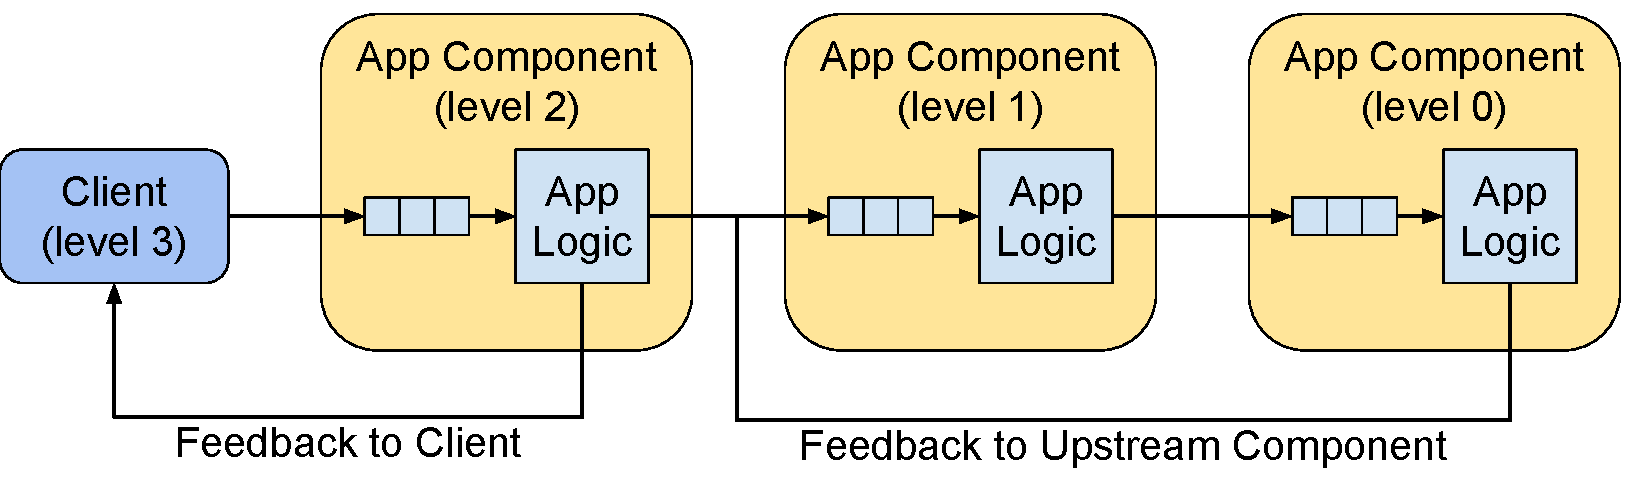
\includegraphics[width=\columnwidth]{figures/oneedge/app_pipeline.pdf}
    \caption{Application Pipeline.}
    \label{fig:app_pipeline}
\end{subfigure}
\begin{subfigure}{.48\columnwidth}
  \centering
    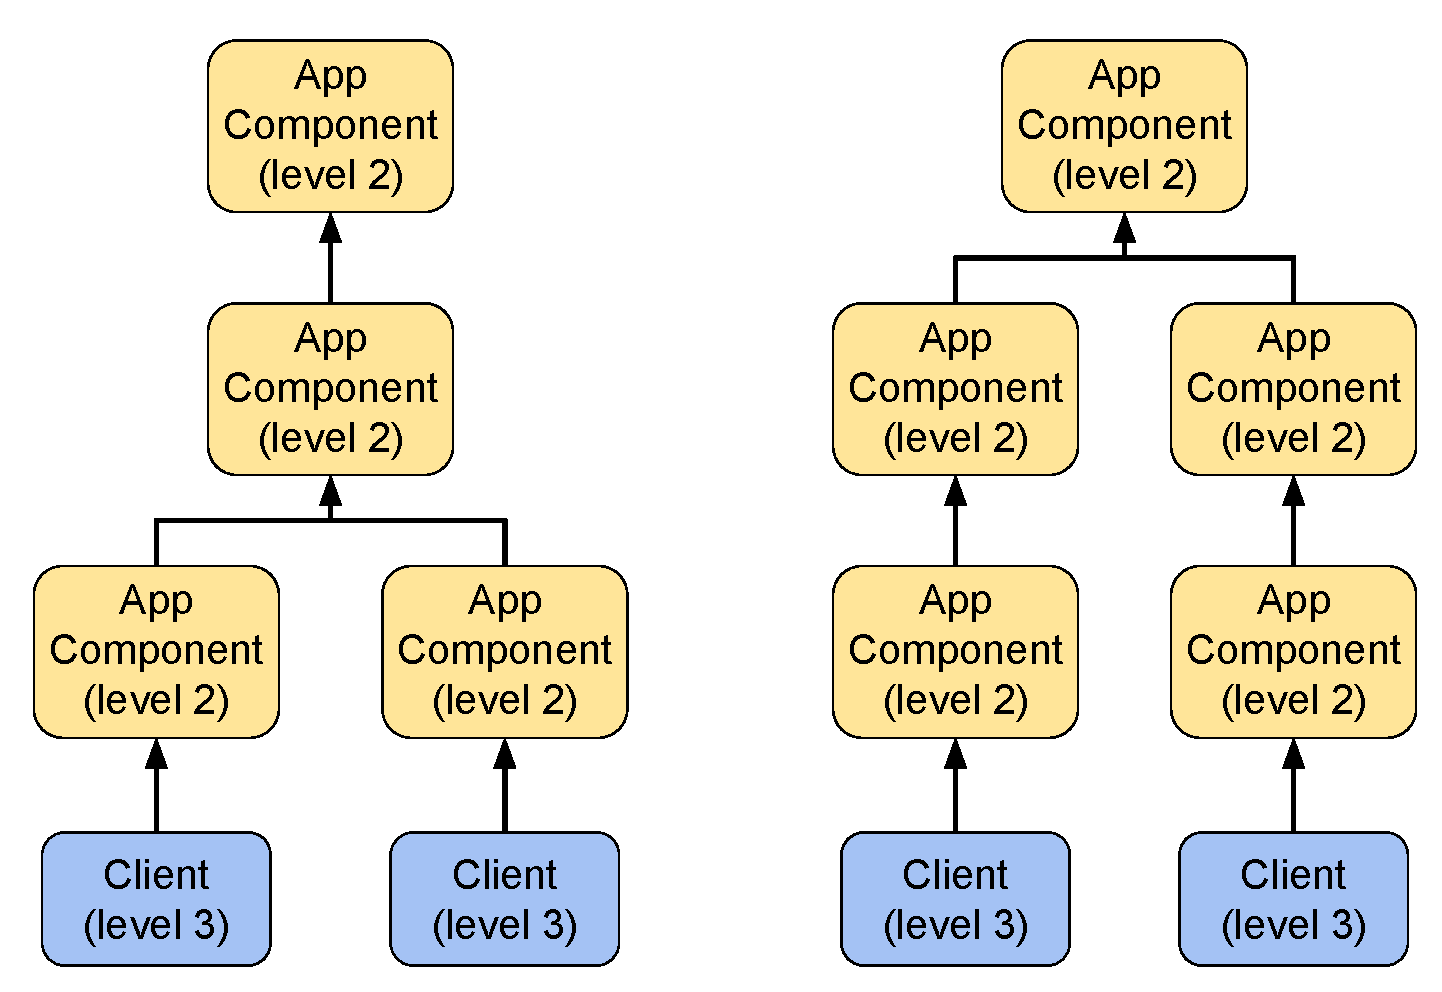
\includegraphics[width=\columnwidth]{figures/oneedge/pipeline_tree.pdf}
    \caption{Actual deployment of a pipeline-based application model resembles a forest with multiple trees.}
    \label{fig:pipeline_tree}
\end{subfigure}
\caption{Description of the application model.}
\label{fig:app_model}
\end{figure}

Although applications are modeled and specified as a linear pipeline, upon deployment for multiple clients, world, the set of application components and the data dependencies among them resemble a forest, as shown in \cref{fig:pipeline_tree}. This is because in order to serve many geo-distributed clients, the same application component needs to have several instances deployed in network proximity of clients so that communication latency to the application instance can be minimized and real-time response made possible. However, not all pipeline components have stringent latency requirements, and thus can serve multiple clients. Each tree in the forest has the most downstream application component (with level 0) as the root node and clients as leaf nodes. Each root-to-leaf path in a tree is a complete application pipeline, and we call each such path except the leaf node an \textit{application instance}. An application component that serves more than one upstream components is essentially processing information gathered from multiple clients, and therefore is able to enable state sharing among clients. However, even for applications that don't share state among clients in their logic, sharing one or more components in the application pipeline among multiple clients can be beneficial. This is because the memory footprint of running multiple independent application components is higher than sharing an application component to serve the same number of clients \todo{quantify?}.

\begin{figure}[ht]
\centering
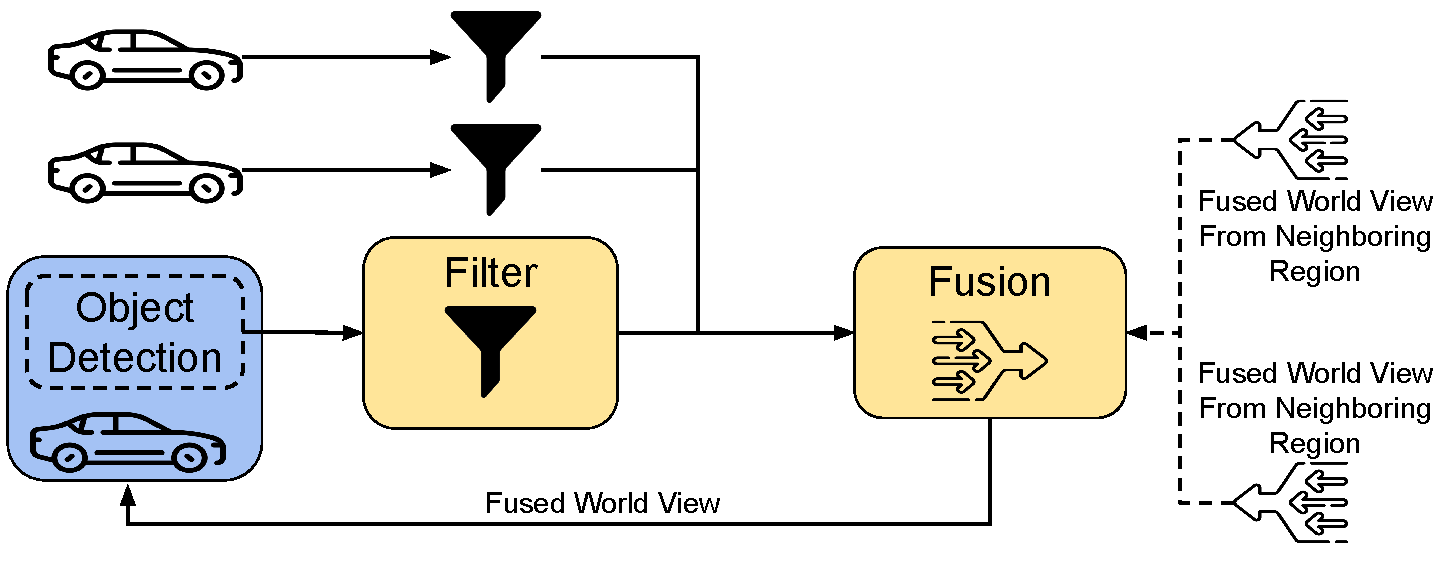
\includegraphics[width=0.8\columnwidth]{figures/oneedge/collaborative_driving_app.pdf}
\caption{The collaborative driving assistance application modeled as a pipeline of components.}
\label{fig:collab_driving_pipeline}
\end{figure}

\par For example, the Collaborative Driving Assistance application can be modeled as a pipeline of application components as shown in \cref{fig:collab_driving_pipeline}. The Client component performs object detection on an input LiDAR sensor stream to generate a list of objects that it can see in its immediate field of view. The Sub-Regional View component aggregates the individual views from multiple vehicles that are in close spatial proximity of one another to create a composite view. This composite view is fed back to the vehicles so that they can improve their lane control and collision avoidance decisions. The output of Sub-Regional View components is processed by the Regional View component to perform higher-level analyses across a larger geographical area.

\begin{comment}
\subsubsection{Programming Model}
\begin{table}
\caption{Programming model API:  communication primitives.}
\label{table:comm_api}
\centering
\resizebox{0.95\textwidth}{!}{%
\begin{tabular}{|c|c|}
\hline
\textbf{Interface} & \textbf{Description} \\ \hline
\begin{tabular}{@{}c@{}} void send\_up (message m, edgeId o) \end{tabular} & \begin{tabular}{@{}c@{}} Sends a message asynchronously from a node \\ to the downstream node connected through edge \textit{o}. \end{tabular} \\ \hline
\begin{tabular}{@{}c@{}} void send\_down (message m, edgeId i,\\ \textbf{optional } nodeId n) \end{tabular} & \begin{tabular}{@{}c@{}}Sends a message asynchronously to all upstream \\nodes connected through edge \textit{i}.  Optionally it can \\ choose to only contact  one of the upstream nodes \textit{n}. \end{tabular} \\ \hline
\begin{tabular}{@{}c@{}} void send\_to (message m, \\nodeId destination) \end{tabular} & \begin{tabular}{@{}c@{}}Sends a message to a specific destination node.
\end{tabular} \\ \hline
\begin{tabular}{@{}c@{}} void send\_to\_partion\_clients (message m, \\partitionId id) \end{tabular} & \begin{tabular}{@{}c@{}}Sends a message to all the clients in a logical partition.
\end{tabular} \\ \hline
\end{tabular}
}
\end{table}
\end{comment}

\subsection{Control-Plane Policies for Application Orchestration}
Effective orchestration of situation-awareness applications on Edge infrastructure requires two main decisions that need to be taken by the control-plane. These two decisions are (i) mapping clients to application instances, and (ii) deploying and managing resources for application instances on Edge sites.

\subsubsection{Mapping Clients to Application Instances}
\newcommand{\clientset}{\mathcal{C}}
\newcommand{\instanceset}{\mathcal{I}}
\newcommand{\resourceset}{\mathcal{R}}

We now formally describe the decision concerning mapping clients to application instances for a specific application. Let $\clientset$ denote the set of clients for the given application and $\instanceset$ denote the set of running instances of all the components of this application. As mentioned before, each application component in $\instanceset$ as well as each client in $\clientset$ has an associated level, which indicates the stage number in the pipelined application model. The mapping of clients and upstream application components to downstream components is defined by a function $\mathcal{M}$, defined in \cref{eq:mapping_domains_eqns} and \cref{eq:mapping_eqn}.
\begin{equation}
\label{eq:mapping_domains_eqns}
\mathcal{M} : \left( \clientset \cup \instanceset \right) \times Z^+ \rightarrow \instanceset
\end{equation}

\begin{equation}
\label{eq:mapping_eqn}
\mathcal{M} \left( c, l \right) = \text{App Component of level }l \text{ serving }c
\end{equation}
The control-plane needs to compute such a mapping so as the ensure that the application requirements discussed in \cref{sec:oneedge_app_reqs} are satisfied.

\subsubsection{Deployment of Application Instances on Edge Sites}
Each application instance, comprising of all the components in the application's pipelined model, need to be deployed on a compute resource. The placement of application components ($\instanceset$) on the set of compute resources ($\resourceset$) can be represented by the function $\mathcal{P}$, as described in \cref{eq:placement_domain_eqn} and \cref{eq:placement_eqn}.

\begin{equation}
\label{eq:placement_domain_eqn}
\mathcal{P} : \instanceset \rightarrow \resourceset
\end{equation}

\begin{equation}
\label{eq:placement_eqn}
\mathcal{P} \left( a \right) = \text{Compute resource hosting }a
\end{equation}
The placement of application components is computed in a manner that meets the end-to-end latency requirements of the application, as described in \label{sec:oneedge_app_reqs}.

\subsection{Application Requirements}
\label{sec:oneedge_app_reqs}
We now discuss the requirements that \oneedge{} allows application developers to specify which allow the application
\begin{figure}
	\centering
	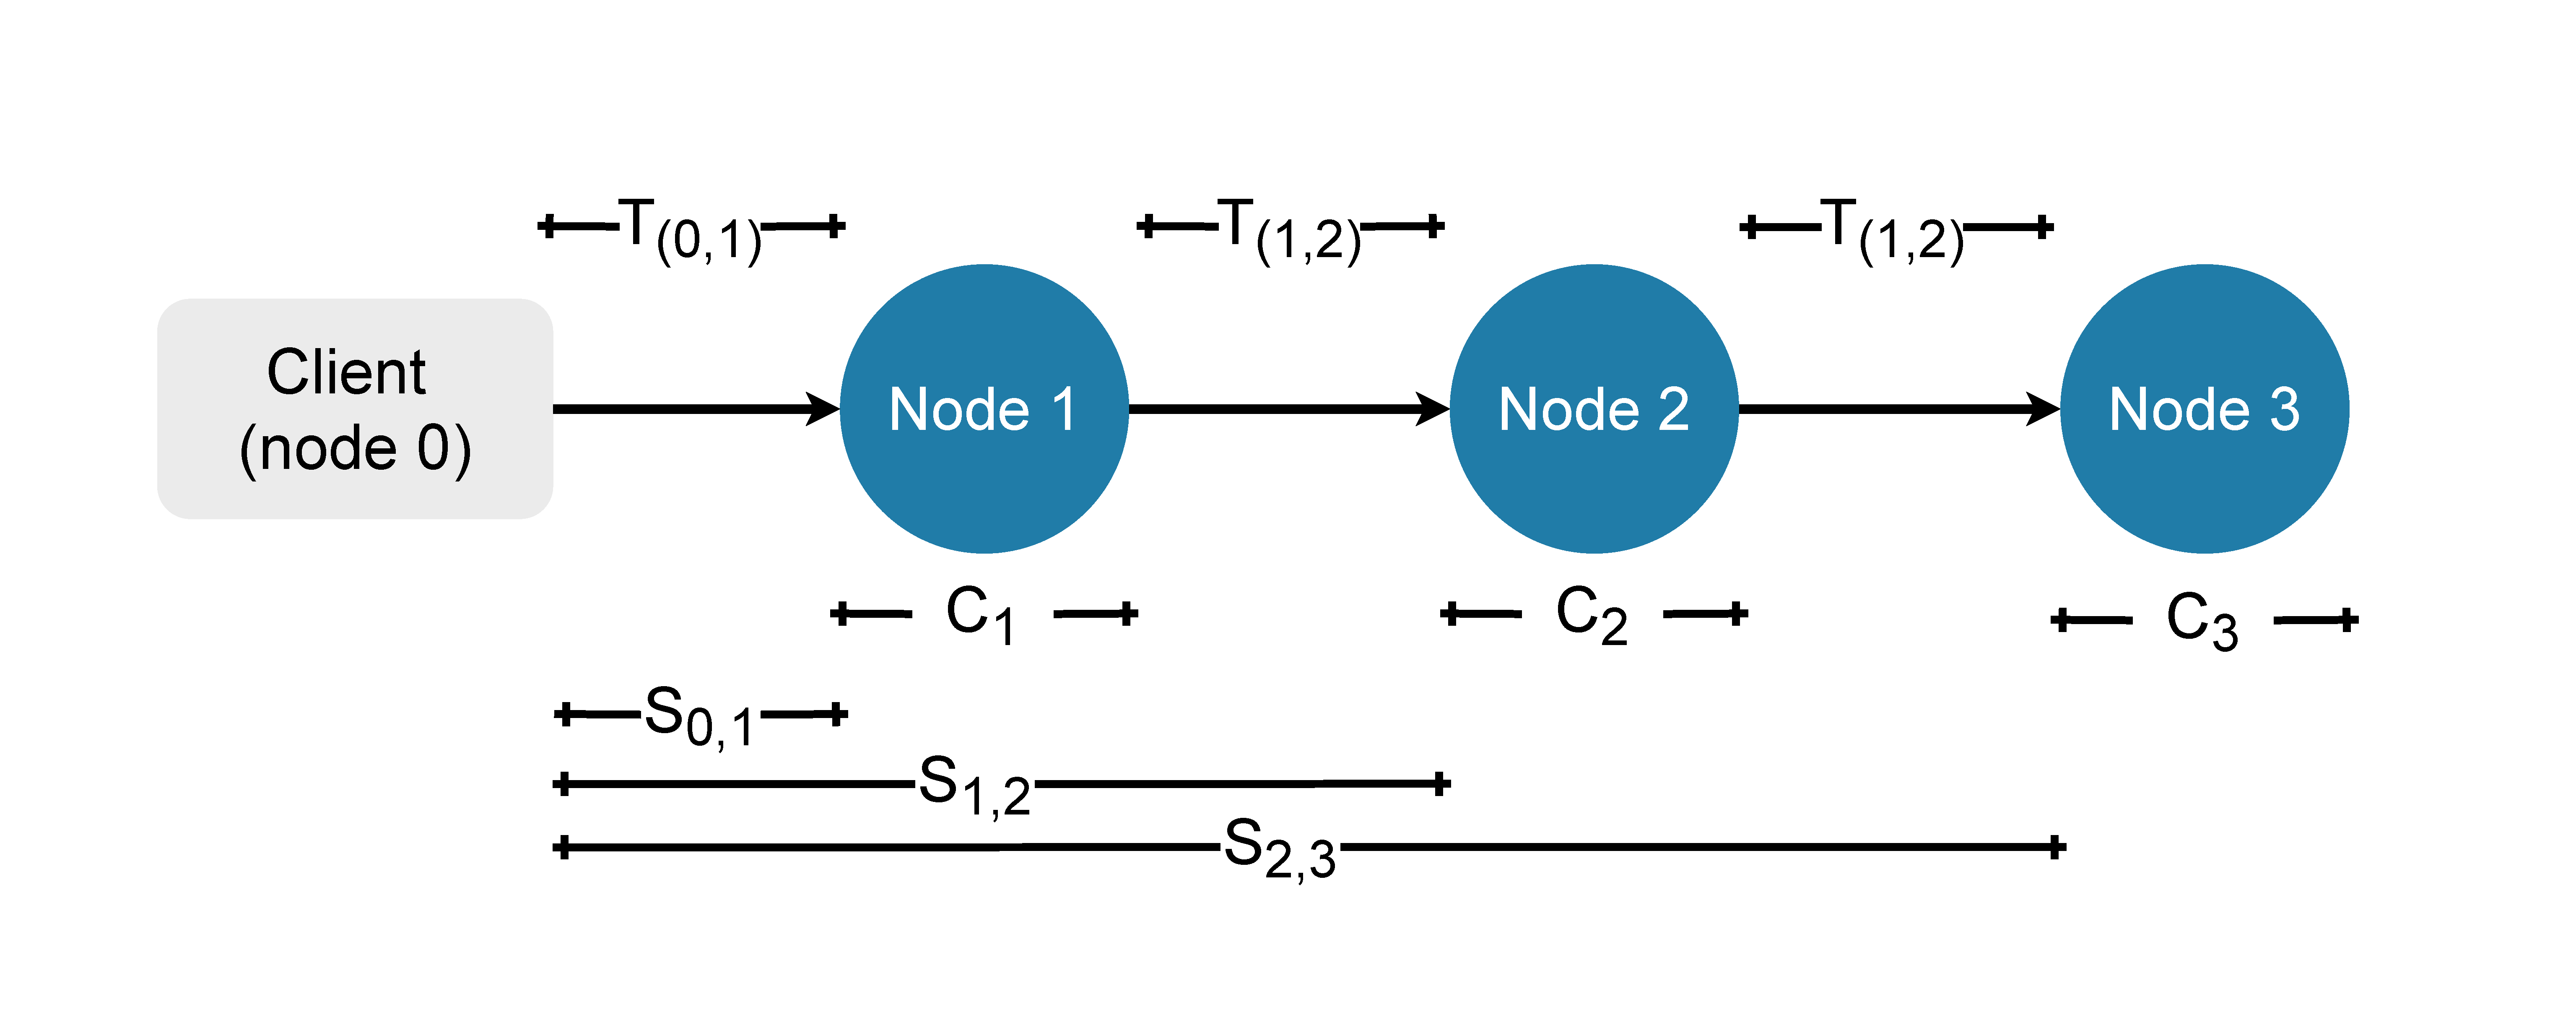
\includegraphics[width=0.95\textwidth]{figures/oneedge/pipeline_latency.pdf}
    \caption{
    A generic pipeline that explains the different components of the tolerable latency staleness. $S_{(i-1,i)}$ is the acceptable latency starting at the output of the client to the input of the node $i$. It is composed of both computational latency $C_j$ and transmission latency $T_{j-1,j}$.}
	\label{fig:pipeline_lat}
\end{figure}

\subsubsection{End-to-End Processing Latency}
Application developers are able to specify the end-to-end processing latency for each component in the application pipeline model. End-to-End processing latency for an application component is the time elapsed between when a specific data-item/event is generated by the client to when it is processed by the application component. This includes the network transmission latency and processing time of all the upstream components. The end-to-end latency constraint for each application component should be satisfied for each client of the given application. The end-to-end latency for client $c$ at application component with level $l$ is defined in \cref{eq:e2e_proc_latency}, which is calculated recursively using the value for the upstream component with level $l+1$. The base case is when the level $l$ equals the level corresponding to the client itself, in which case, the end-to-end latency is equal to the processing latency on the client.
\begin{equation}
\label{eq:e2e_proc_latency}
E2E \left( c, l \right) = E2E \left(c , l+1 \right) + proc \left( \mathcal{M} \left( c, l \right) \right) + net \left(  \mathcal{M} \left( c, l+1 \right) , \mathcal{M} \left( c, l \right) \right)
\end{equation}

\subsubsection{Spatial Affinity}
Several situation-awareness applications such as the collaborative driving assistance application (\cref{fig:collab_driving_pipeline}) consist of components that are tied to a specific geographical area, and are meant to serve clients located in that geographical area only. This is meant to enable information sharing between clients that are in close spatial proximity to one another. We denote the geographical area served by an application component as its \textit{spatial context}. The partitioning of the geographical space into spatial contexts is application-specific. More precisely, the application developer would specify a function $\mathcal{S}$ that maps a geographical location $\left( x , y \right)$ to a unique spatial context $s_z$ (identified by a positive integer $z$) (\cref{eq:spatial_context}).

\begin{equation}
\label{eq:spatial_context}
   \mathcal{S}: X \times Y \rightarrow \{ s_0, s_1, \cdots \}
\end{equation}
\begin{equation}
   X = \{x \in \mathbb{R}~|~-\pi < x < \pi\}
\end{equation}
\begin{equation}
   Y = \{y \in \mathbb{R}~|~\dfrac{-\pi}{2} < y < \dfrac{\pi}{2}\}
\end{equation}

For an application component of level $l$ that needs to facilitate inter-client information sharing, the control-plane assigns each spatial context $s_z$ with an application component and map all clients located within that spatial context to that instance. Multiple spatial contexts can also be mapped to the same application instance. However, the main requirement is that all clients within given spatial context should be served by the same application instance so that they can effectively share state with other clients in the same spatial context. The quality of this client-application-instance mapping is quantified using the Spatial Alignment metric, as shown in \cref{eq:spatial_alignment}. The Spatial Alignment metric is defined for each spatial context $s_z$ that is served by the application component instance $a$ at level $l$.  Ideally, the spatial alignment metric should be equal to 1 for all spatial contexts.
\begin{equation}
\label{eq:spatial_alignment}
SA \left( a \right) = \dfrac{|\{ c \in \clientset : c.loc \in s_z   \mathcal{M} \left( c, l\right) = a \}|}{|\{ c \in \clientset : c.loc \in s_z \}|}
\end{equation}
\todo{Can we connect application instance $a$ with $s_z$?}

\subsection{Workload Dynamism}

\subsubsection{Client Mobility}
Typical situation-awareness applications have clients that are inherently mobile, for example, vehicles, pedestrians, UAVs, etc. The mobility of clients creates two main challenges. For applications involving inter-client information sharing, the mapping of a client to an instance of a given component is based on the spatial context of that component's instance and the location of the client. Due to client mobility, the client's location might change so much that it exits the spatial context of the current application component instance, and thus is not able to coordinate with the correct subset of other clients that are in its physical proximity. This requires that the client be migrated to the application component instance that has the correct spatial context which corresponds to the current location of the client. Secondly, client mobility can result in a change in the network routing and hence communication latency to and from the application instance. This change in communication latency affects the end-to-end processing latency for that client's data by the current application instance. This necessitates that the client be migrated to an application instance that can satisfy the end-to-end latency requirements.

\subsubsection{Changes in Processing Requirements of Applications}
The frequency of events generated by different application components in an application pipeline changes over time. This is either due to the mobility of clients which changes the properties of the environment sensed by the clients. For instance, in the Collaborative Driving Assistance application, the number of neighboring vehicles output by the Detection component (in the client) is a function of the density of neighboring traffic, which changes with time as the ego vehicle moves. The change in processing requirements of applications can also happen for static sensors, such as CCTV cameras, when the environment they are sensing undergoes changes. For instance, in the \todo{} application, the frequency of events generated by the \todo{} component depends on the number of cars in the field-of-view of a camera, which changes over time.

\section{Architectural Components of \oneedge{}}

\subsection{Client Library}

\subsection{Site Manager}

\subsection{Controller}

\section{Spatial-Affinity-aware Application Scheduling using Dynamic Spatial Context Management}

\subsection{Flexible Partitioning of Geographical Space}

\subsection{Control-Plane Policy for Spatial-Affinity-aware Application Scheduling}

\section{Latency-aware Application Scheduling using Network Proximity Estimation}

\subsection{Deployment of Network Coordinate Agents}

\subsection{Estimating End-to-End Processing Latency}

\subsection{Control-Plane Policy for Latency-aware Application Scheduling}

\section{Distributed Monitoring in \oneedge{}}

\section{Implementation}

\section{Evaluations}

\section{Conclusion}